% Author: Izaak Neutelings (November 2020)
\documentclass[border=3pt,tikz]{standalone}
\usepackage{physics}
\usepackage{tikz}
\usepackage[outline]{contour} % glow around text
\usetikzlibrary{patterns,decorations.pathmorphing}
\usetikzlibrary{decorations.markings}
\usetikzlibrary{arrows.meta}
\usetikzlibrary{calc}
\tikzset{>=latex}
\contourlength{1.1pt}

\colorlet{mydarkblue}{blue!40!black}
\colorlet{myblue}{blue!70!black}
\colorlet{myred}{red!65!black}
\colorlet{myorange}{orange!90!black!90}
\colorlet{vcol}{green!45!black}
\colorlet{watercol}{blue!80!cyan!10!white}
\colorlet{darkwatercol}{blue!80!cyan!80!black!30!white}
\colorlet{metalcol}{blue!25!black!30!white}
\tikzstyle{piston}=[blue!50!black,top color=blue!30,bottom color=blue!50,middle color=blue!20,shading angle=0]
\tikzstyle{water}=[draw=mydarkblue,rounded corners=0.1,top color=watercol!90,bottom color=watercol!90!black,middle color=watercol!50,shading angle=20]
\tikzstyle{horizontal water}=[water,top color=watercol!90!black!90,bottom color=watercol!90!black!90,middle color=watercol!80,shading angle=0]
\tikzstyle{metal}=[draw=metalcol!10!black,rounded corners=0.1,top color=metalcol,bottom color=metalcol!80!black,shading angle=10]
\tikzstyle{vvec}=[->,very thick,vcol,line cap=round]
\tikzstyle{force}=[->,myred,very thick,line cap=round]
\tikzstyle{width}=[{Latex[length=4,width=3]}-{Latex[length=4,width=3]}]
\def\tick#1#2{\draw[thick] (#1)++(#2:0.12) --++ (#2-180:0.24)}

\begin{document}


% LAMINAR FLOW LAYERS
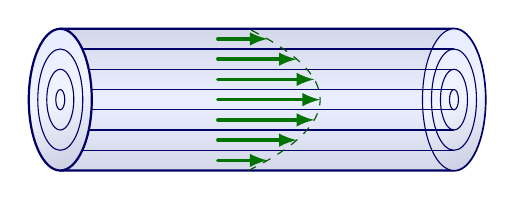
\begin{tikzpicture}
    \def\L{5.0}   % total length
    \def\Rx{0.40} % big pipe vertical radius right
    \def\Ry{0.90} % big pipe vertical radius right
    \def\v{1.3}   % velocity magnitude
    \def\N{3}     % velocity magnitude

    % WATER
    \draw[horizontal water,thick]
    (0,\Ry) -- (0,-\Ry)  coordinate (A1) --++ (\L,0) arc(-90:90:{\Rx} and \Ry) -- cycle;
    \draw[water]
    (\L,0) ellipse({\Rx} and \Ry);

    \draw[water]
    (0,0) ellipse({\Rx} and \Ry);
    %\draw[horizontal water,line width=0.1] %draw=none
    %  (0,-\Ry) rectangle (\L,\Ry);
    \foreach \i [evaluate={\x=(\i-0.5)/(\N+0.5)}] in {1,...,\N}{
            \draw[mydarkblue] %,line width=0.05
            (0,0) ellipse({\x*\Rx} and \x*\Ry)
            (\L,0) ellipse({\x*\Rx} and \x*\Ry);
            \draw[mydarkblue] %,dashed]  %,line width=0.05
            (0, \x*\Ry) --++ (\L,0)
            (0,-\x*\Ry) --++ (\L,0); %arc(90:-90:{\x*\Rx} and \x*\Ry) --++ (-\L,0);
        }
    %\draw[horizontal water,draw=none]
    %  (0,{-\N/(\N+1)*\Ry}) rectangle (\L,{\N/(\N+1)*\Ry});
    \draw[water,thick]
    (0,0) ellipse({\Rx} and \Ry);
    \foreach \i [evaluate={\x=(\i-0.5)/(\N+0.5)}] in {1,...,\N}{
            \draw[mydarkblue] (0,0) ellipse({\x*\Rx} and \x*\Ry);
        }
    %\draw[mydarkblue,thick]
    %  (0,\Ry) arc(90:-90:{\Rx} and \Ry) coordinate (A1) --++ (\L,0) arc(-90:90:{\Rx} and \Ry) -- cycle;
    \draw[vcol!70!black,dashed,samples=100,smooth,variable=\y,domain=-1:1]
    plot({0.4*\L+\v*(1-0.7*\y*\y)},\y*\Ry);
    \draw[vvec] (0.4*\L,0) --++ (\v,0);
    \foreach \i [evaluate={\y=(\i)/(\N+0.5); \vy=\v*(1-0.7*\y^2);}] in {1,...,\N}{
            \draw[vvec] (0.4*\L, \y*\Ry) --++ (\vy,0);
            \draw[vvec] (0.4*\L,-\y*\Ry) --++ (\vy,0);
        }

\end{tikzpicture}
\end{document}